\documentclass{standalone}

\usepackage{tikz}

\usepackage{helvet}

\usetikzlibrary{shadows}

\begin{document}
	
	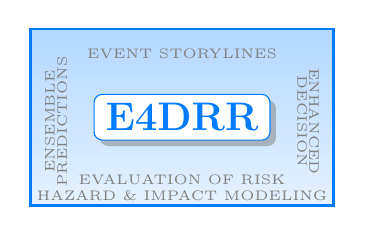
\begin{tikzpicture}[scale=0.8, font=\sffamily]
		
		\def\W{4.8} % Width of the rectangle
		
		\def\H{2.8} % Height of the rectangle
		
		% Define colors
		
		\definecolor{logoBlue}{RGB}{0,123,255}
		
		\definecolor{logoGray}{RGB}{128,128,128}
		
		% Draw the rectangle with gradient background
		
		\shade[top color=logoBlue!30, bottom color=logoBlue!10] (0,0) rectangle (\W,\H);
		
		% Define a smaller font size
		
		\newcommand{\tinysmall}{\fontsize{3}{3.6}\selectfont}
		
		\newcommand{\supertinysmall}{\fontsize{0.8}{1.4}\selectfont}
		
		% Draw a rounded rectangle border around E4DRR
		
		\node[draw=logoBlue, fill=white, rounded corners=3pt, align=center, text width=2cm, font=\bfseries\Large, text=logoBlue, drop shadow] at (\W/2,\H/2) {E4DRR};
		
		% Position the phrases around E4DRR
		
		\node[align=center, font=\tinysmall, text=logoGray] at (\W/2, \H-0.4) {EVENT STORYLINES};
		
		\node[align=center, font=\tinysmall, text=logoGray] at (\W/2, 0.4) {EVALUATION OF RISK};
		
		\node[align=center, font=\tinysmall, text=logoGray] at (\W/2, 0.15) {HAZARD \& IMPACT MODELING};
		
		\node[align=center, font=\supertinysmall, text=logoGray, rotate=90] at (0.4, \H/2.1) {ENSEMBLE \\ PREDICTIONS};
		
		\node[align=center, font=\supertinysmall, text=logoGray, rotate=-90] at (\W-0.4, \H/2.1) {ENHANCED \\ DECISION};
		
		% Draw a border line around the logo
		
		\draw[logoBlue, line width=1pt] (0,0) rectangle (\W,\H);
		
	\end{tikzpicture}
	
\end{document}